\subsection{
  Step 2: Calculating \(Xsqr\)
}
This step corresponds to the following Futhark code:
\begin{figure}[H]
    \centering
    \ehaskell[firstline=117,lastline=118]{../src/fut-handout/bfast-distrib.fut}
    \caption{Futhark function for generating X.}
    \label{fut:kernel2}
\end{figure}
%We recall that the dimensions of \(X\) are \texttt{[k2p2][N]}, and thus, the
%dimensions of \(X^T\) are \texttt{[N][k2p2]}.

The \texttt{matmul\_filt} function, as it is used here, calculates the product
of the two input matrices \(Xh\) and \(Xh^T\), while additionally taking a
filtering vector of length \(n\) as input, corresponding to a row from \(Yh\).
In this vector, the value of its \(k\)th element determines whether the product
\(Xh_{ik}Xh^T_{kj}\) is to be excluded from the summation
\(\sum\limits_{a=0}^{n-1} Xh_{ia}Xh^T_{aj}\) when calculating some element
at row \(i\), column \(j\) in the output matrix.
% XXX: The semantics could be written in a cooler fashion by writing the
% summation over products X_{bla}X^T_{bla2}*f_k where f_k is 0 when kth elem in
% filt vector is NAN and 1 otherwise
Since \(Xh\) has dimensions \texttt{[k2p2][n]}, the output matrix from each call
to \texttt{matmul\_filt} will have dimensions \texttt{[k2p2][k2p2]}.
Since we perform this calculation for every one of the \(m\) rows in \(Y\), the
output, \(Xsqr\), has shape \texttt{[m][k2p2][k2p2]}.

These semantics can naively be replicated in a CUDA-kernel with grid size \(m\)
and block size \( (k2p2, k2p2)\), in which the \(k\)th block performs one
matrix-matrix multplication with row \(k\) from \(Y\) as its filtering vector,
and each thread in a block is responsible for calculating one element in the
output matrix.
This naive approach is implemented in the \texttt{bfast\_step\_2} kernel in
\texttt{kernels/bfast\_step\_2.cu}.

C-like pseudocode for how this kernel works can be seen below:
\begin{minted}{c}
for (int i = 0; i < m; i++) {           // blockIdx.x
  for (int y = 0; y < k2p2; y++) {      // threadIdx.y
    for (int x = 0; x < k2p2; x++) {    // threadIdx.x
      float accum = 0.0;
      for (int l = 0; l < n; l++) {     // sequential
        if (!isnan(Yh[i,l])) {
          accum += Xh[y,l] * Xth[l,x];
        }
      }
      Xsqr[i, y, x] = accum;
    }
  }
}
\end{minted}
% corollary 2, safe to interchange inwards

We observe that there is great opportunity for optimizing locality, since we
have many global memory accesses to the same elements of both \(X\), \(Xth\)
and \(Yh\).
To carry out this optimization, we will apply the tiling technique, which
involves stripmining relevant loops and interchanging them inwards.

The first step is to stripmine the outermost loop with a tile size \texttt{T},
as seen below:
\begin{minted}[linenos]{c}
for (int i = 0; i < m; i += T) {          // blockIdx.x
  for (int ii = 0; ii < T; ii++) {        // stripmined loop
    for (int y = 0; y < k2p2; y++) {      // threadIdx.y
      for (int x = 0; x < k2p2; x++) {    // threadIdx.x
        float accum = 0.0;
        for (int l = 0; l < n; l++) {     // sequential
          if (!isnan(Yh[i+ii,l])) {
            accum += Xh[y,l] * Xth[l,x];
          }
        }
        Xsqr[i+ii, y, x] = accum;
      }
    }
  }
}
\end{minted}
This transformation is always safe to apply. When the optimization is done, a
suitable value of \texttt{T} can be found that best optimizes performance.

The next step is to interchange the stripmined loop inwards.
To show that this is a valid transformation, we must show that the interchange
does not cause any direction vector to become invalid.
In the code above, we can easily see that there is only one dependency, which
is the one that arises from reading from and writing to the variable
\texttt{accum}.
Since we only read from \texttt{Yh}, \texttt{Xh}, and \texttt{Xth}, the
statements involving these arrays do not cause dependencies to arise.
We can also easily see that the write to \texttt{Xsqr} does not cause a WAW
dependency to arise, since every iteration writes to a new index of this array.
Looking at the \texttt{accum}-dependency arising from the increment in the
statement on line 8, we see that this is a dependency with direction \texttt{<}
in the innermost loop, since we read the value that was written in the previous
iteration.
Since \texttt{accum} is private to the second-most inner loop, the direction is
\texttt{=} for all loops but the innermost.
Thus, since the dependency has direction vector \texttt{[=,=,=,=,<]}, we see
that it is impossible for us to cause this direction vector to become invalid,
and we are free to interchange the loops as we wish, as per theorem 7 in
\cite{pmph}.

Interchanging the stripmined loop inwards gives us:
\begin{minted}[linenos]{c}
for (int i = 0; i < m; i += T) {          // blockIdx.x
  for (int y = 0; y < k2p2; y++) {        // threadIdx.y
    for (int x = 0; x < k2p2; x++) {      // threadIdx.x
      for (int ii = 0; ii < T; ii++) {
        float accum = 0.0;
        for (int l = 0; l < n; l++) {     // sequential
          if (!isnan(Yh[i+ii,l])) {
            accum += Xh[y,l] * Xth[l,x];
          }
        }
        Xsqr[i+ii, y, x] = accum;
      }
    }
  }
}
\end{minted}

Next, we wish to distribute the stripmined loop across the contents of its
body.
Consider the dependency graph for the body of the stripmined loop, as sketched
on \ref{fig:step-2-graph}.
We see that each of the three nodes makes up its own strongly connected
component, and it is thus, by theorem 9 (\cite{pmph}), legal to distribute the
loop.
\begin{figure}[H]
    \centering
    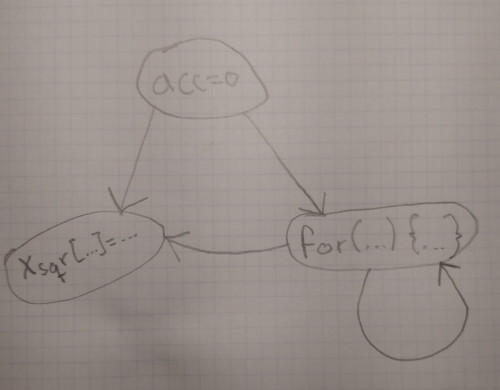
\includegraphics[width=0.4\textwidth]{step-2-graph.jpg}
    \caption{Dependency graph for the contents of the \texttt{ii}-loop}\label{fig:step-2-graph}
\end{figure}
Since \texttt{accum} is declared inside the loop we are distributing, we
must perform array expansion on this variable.
The result of the loop distribution can be seen below:
\begin{minted}[linenos]{c}
for (int i = 0; i < m; i += T) {        // blockIdx.x
  for (int y = 0; y < k2p2; y++) {      // threadIdx.y
    for (int x = 0; x < k2p2; x++) {    // threadIdx.x
      float accum[T];
      for (int ii = 0; ii < T; ii++) {
        accum[ii] = 0.0;
      }
      for (int ii = 0; ii < T; ii++) {
        for (int l = 0; l < n; l++) {
          if (!isnan(Yh[i+ii,l])) {
            accum[ii] += Xh[y,l] * Xth[l,x];
          }
        }
      }
      for (int ii = 0; ii < T; ii++) {
        Xsqr[i+ii, y, x] = accum[ii];
      }
    }
  }
}
\end{minted}

We observe that the \texttt{accum}-dependency on line 11 now has direction
vector \texttt{[=,=,=,<,=]}.
We can thus interchange the \texttt{l}-loop on line 9 with the surrounding
\texttt{ii}-loop on line 8, and we get the following:
\begin{minted}[linenos]{c}
for (int i = 0; i < m; i += T) {        // blockIdx.x
  for (int y = 0; y < k2p2; y++) {      // threadIdx.y
    for (int x = 0; x < k2p2; x++) {    // threadIdx.x
      float accum[T];
      for (int ii = 0; ii < T; ii++) {
        accum[ii] = 0.0;
      }
      for (int l = 0; l < n; l++) {
        for (int ii = 0; ii < T; ii++) {
          if (!isnan(Yh[i+ii,l])) {
            accum[ii] += Xh[y,l] * Xth[l,x];
          }
        }
      }
      for (int ii = 0; ii < T; ii++) {
        Xsqr[i+ii, y, x] = accum[ii];
      }
    }
  }
}
\end{minted}

















